\chapter{H-Bridge}

\section{Introduction}
The control of two motors has been considered a high priority task in the robot design,due to the decision of contructing a H-bridge circuit from scratch.It can be considered a risky and labourious choice,infact it could be easier buy a motor-driven IC (LMD18200 H-Bridge),on the other hand has been considered educationally interesting designing our own motor driver.H-Bridge circuit is a very common circuit used to control the direction of a motor (applying an high signal to one of the input pins,infact reversing the current flow trought the motor is possible change the spinning direction),moreover it is possible control the speed of the motor by PWM signal.


\section{Components choice and design implementation}
\label{sec:H-bridge_schematics}
Designing an H-Bridge may appear a simple task,in general it is a rather simple circuit,containing four switching elements and the load in the center,however many small factors have to be considered that,if under estimed,could partially damage or,in the worst case,destroy the components and circuits connected.Given the recent reasons,excess of zeal has been put in components choice,furthermore different design options has been considered and tested before obtaining a fully working H-bridge (figure \ref{fig:bridge}) and reliable in terms of robustness.Before going through the components selection and analysis some 
details about the mode of operation of H-bridge have to be specified:as briefly explained above,this kind of motor driver consists in four switching elements,in an H-like configuration.It is possible divide it in  two side,working in an equivalent way but they cannot,for different reasons clarified below,being turned on in the same moment.Each "side" is composed by an "high circuit" called source, this name originates from its function which is to be a source for the load;a "below circuit" called sink,which provides a channel for the current flow from the source through the load.For the source circuit is usually used p-channel transistor,whereas n-channel is used for sink one.It can be possible use two n-channel,but it become difficult control it in the source.

\begin{figure}[!ht]
	\begin{subfigure}{.49\textwidth}
		\centering
		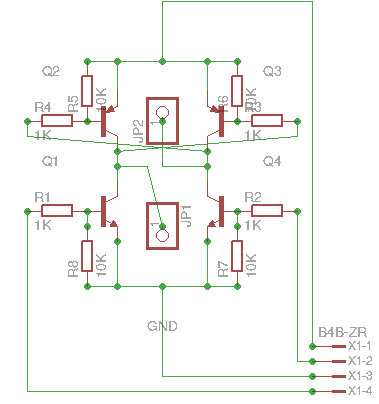
\includegraphics[width=1\textwidth]{figures/H-bridge_schematics}
		\caption{Schematics}
		\label{fig:1-bridgeSCH}
	\end{subfigure}
	\begin{subfigure}{.49\textwidth}
		\centering
		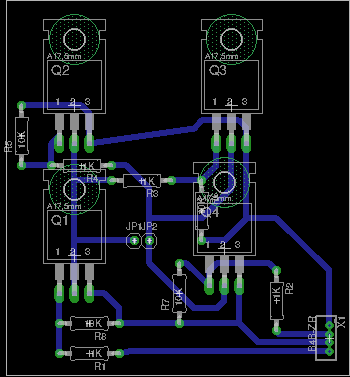
\includegraphics[width=1\textwidth]{figures/H-bridge_board}
		\caption{Boards}
		\label{fig:1-bridgeBRD}
	\end{subfigure}
\caption{The H-Bridge board}
\label{fig:bridge}
\end{figure}


The key decision to make for an H-Bridge is the selection of switching elements.Main factors that has affected the components choice are the operating current and the operating voltage;since the main aim is not an accurate speed control,switching frequency has not been considered a big concern and,in the end,power efficiency is not a big concern for this kind of application,heat is.Since transistor,when operated as switch it has two states:on and off.In the "on" state it behaves like a small resistor (called channel resistance and denote as $ r_{dson} $ for MOSFET,$ r_{tr} $ for BJT),the loss on it is converted in heat to dissipate,so the lower $ r_{dson} $/$ r_{tr} $is better.Keeping in mind the above criteria,MOSFET,BJT and IGBT transistors can be used as switching elements.Since the employed motors are low power Micro Gearmotors (1600 mA-12V)DC reversible,IGBTs have not been considered.MOSFETs are usually preferred in H-bridge construction,they offer a good response time to switching signal,low power dissipation (IRF630 has $ r_{dson}=0.4\Omega $,$ V_{gs}=10V $-$ I_{D}=5.4A $ test conditions) and large gate lead input impedances ($\geq10^{14}\Omega$),but then they are extremely fragile and voltage driven,it means that for an efficient motor driver,in terms of control,it is necessary a large span of input voltage.Infact referring to IRF630/IR9630 (this couple of MOSFET has been considered meanwhile choosing the different components) output characteristic at working temperature $ T=25^\circ C $(fig2)(it has been presumed that the reader is familiar with transistor theory)the minimun voltage difference between the gate and source terminal (to let the MOSFET work in Ohmic Region) is 4.5V and,keeping in mind that MOSFET is influenced by gate-source voltage but hardly at all influenced by drain-source voltage $ V_{ds} $,to assure that the switch is turned on and a relevant current flowing through the motor is necessary $ V_{gs}=15V $,making necessary a conditioning circuit to amplify the PWM signal (+3.3V) from the FPGA,not a big issue but,being tight on time, more workload and details to consider.In view of these considerations,it has settled to use BJT,this kind of transistor,similarly to MOSFET, comes in either \emph{npn} or \emph{pnp},differently it is a current driven device,infact a small input current and voltage at its base allows to control a much larger collector-to-emitter current,fitting perfectly our application case and avoiding any kind of conditioning circuit for the PWM signal generated through FPGA.Infact the flowing current through collector and emitter is proportionally larger to the input one,the relationship between them is called gain of transistor an labeled $h_{fe}$,but it does not mean that the transistor is "genereting" current,what it does is "resist less".This behavior is described by the fundamental formula of BJT: $I_C=h_{fe}\cdot I_B$,every transistor has its own unique $h_{fe}$ and it is taken to be a constant (typically around 10 to 500),but it may change slightly with the temperature and with the collector-to-emitter voltage.To keep in mind choosing the right BJT transistor is that it causes a voltage drop between collector and emitter when saturated ($V_{ce}(sat)$,usually around 0.2 V to 1 V),responsable of power dissipation, and between base and emitter junction($V_{be}$).This last voltage difference is important when calculating the current flow "into" the base and the input resistor value.Given all the constraints,the TIP1xx Darlington BJT family has proved to be the best choice for this project.Darlington transistor (called Darlington pair,figure \ref{fig:darlington}) consists in two BTJ attached together,with the advantage of a wider $h_{fe}$ than a single BJT ($h_{fe}\approx h_{fe1}\cdot h_{fe1}$)),on the other hand it has slower response times (it takes longet for the top transistor to turn the lower on and off) and twice $V_{be}$.

\begin{figure}[!ht]
	\centering
	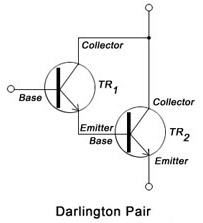
\includegraphics[width=0.5\textwidth]{figures/Darlingtonpair}
	\caption{Darlington transistor pair}
	\label{fig:darlington}
\end{figure}

In particular,TIP102 (\emph{npn} juction) has been chose to implement the sink circuit and TIP107 to implement the source (\emph{pnp} juction),reasons behind this choice are that those two transistors are complementary,and they're supplied with a build-in diode,making not necessary add an extra diode in parallel with the transistors,the role of this diode is very important,infact since the load is a DC motor (inductive load),when the switch is turned off,the electromagnetic field inside the motor has to collapse,but until it happens,current must still flows through the windings,the diode provide a low resistance path for this "collapse" current and thus keep the voltage on the motor terminals within a  reasonable range.Furthermore,TIP102/TIP107 are capable to assure the maximum current flow requested from the Microgear Motor (1600mA,12V) and thanks to they're big DC current gain ($h_{fe}=1000$),a small range of base current is enough to obtain $I_C=1600mA$ (keeping in mind the fundamental formula of the BJT,$I_B=I_C/h_{fe}=1600mA/1000=1,6mA$),keeping at the same time the $V_{be}$ enough low (overall $V_{be}1.4 V$ with $V_{cc}=12 V$).Last relevant characteristic about the chosen transistors is the low collector-emitter current saturation voltage,responsable of the power dissipation and consequently heating.In the implemented H-Bridge,has been preferred driving only the sink base,for the sake of simplicity and for safety reasons,infact to avoid any exposure of the FPGA pins to voltage not designed to handle,the source base has been connected to the collector of the sink,in this way the \emph{pnp} BJT is turned on only when the $ 1k\Omega $ resistor is grounded (it happens when the right side \emph{npn} BJT is turned on),furthermore the $ 10k\Omega $ works as pull-up resistance three-stating the source circuit when the sink is turned off.In an similar way,in the sink circuit the $ 10k\Omega $ resistor ground the \emph{npn} BJT when no there's no input base current and provide an excessive current flowing in the base when the transistor is turned on.On the other hand,with this hardware configuration,implementing the code to control the motor speed and avoid that both the side of the H-Bridge are turned on (due to Darlington pair slow switching frequency,it may be possible that for a small instant transistors on the same side will still be on,causing shoot through with probability of damage to the whole circuit) is more difficult and risky.A suitable solution has been implemented by designing a new circuit  between the H-Bridge and the main board,consisting in a \emph{npn} BJT transistor (TIP102) that connect the H-bridge to the ground and two pins that connect the FPGA to the input pins (figure  \ref{fig:driveH}).

\begin{figure}[!ht]
	\begin{subfigure}{.49\textwidth}
		\centering
		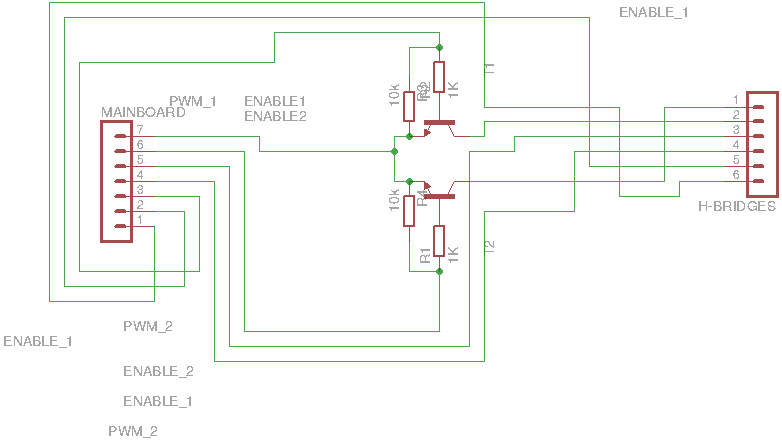
\includegraphics[width=1\textwidth]{figures/drive}
		\caption{Schematics}
		\label{fig:driveSCH}
	\end{subfigure}
	\begin{subfigure}{.49\textwidth}
		\centering
		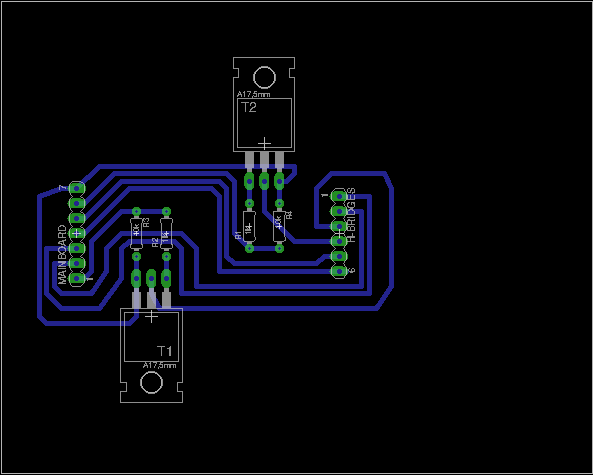
\includegraphics[width=1\textwidth]{figures/drivebrd}
		\caption{Board}
		\label{fig:driveBRD}
	\end{subfigure}
\caption{The H-Bridge drive board}
\label{fig:driveH}
\end{figure}

Thus,the motor speed is controlled through PWM direclty on the "Ground Transistor",that works as bottleneck for the current flowing in the H-bridge,while the H-bridge switch are turned on using an enable signal (0-3.3V) that turns on just one H-bridge side per time is on and avoiding shoot through. \newpage

\section{Conclusions}

Designing an H-Bridge from scratch has not been a simple task and it has been object of different updates during the whole project developement,but it has been educationally interesting,since it has been necessary collecting information about components and examine in depth transistors theory.In the end,we have achieved to build a fully working and robust H-Bridge,allowing a reliable control speed,infact in test condition of $V_{cc}=12 V$ it was possible,through modulating the PWM obtain a smooth motors spinning at different rotation speeds and at the same time we have achieved a good safety level,avoiding any damages to the different components and the whole circuit.